\documentclass[t,aspectratio=169,svgnames]{beamer}
\usepackage[utf8]{inputenc}
\usepackage[T1]{fontenc}

%%%%%%%%%%%%%%%%%%%%%%%%%%%% Wenn ihre Folien auf Deutsch sind (die letzte ist der Default)
\usepackage[english,ngerman]{babel}
\usepackage[autostyle=true,german=quotes]{csquotes}
%%%%%%%%%%%%%%%%%%%%%%%%%%%% for English slides, use this:
%\usepackage[german,english]{babel}
%\usepackage[autostyle=true]{csquotes}

% Theme mit kleinen Anpassungen
\usetheme[progressbar=frametitle]{moloch}
\usecolortheme{default}
\setbeamercolor{title separator}{fg=YellowGreen}
\setbeamercolor{progress bar}{fg=YellowGreen,bg=YellowGreen!15!white}
\setbeamercolor{frametitle}{fg=black,bg=white}
\hypersetup{colorlinks,linkcolor=,urlcolor=YellowGreen!66!black}
\usepackage{appendixnumberbeamer}
\setbeamertemplate{frametitle continuation}{}
\setbeamertemplate{itemize items}[triangle]
\setbeamertemplate{frame footer}{\strut\insertshorttitle{} -- \insertshortauthor{}}


% Fonts
\usepackage[medium]{FiraSans}
\usepackage[medium]{FiraMono} % für code
\usepackage{newtxsf} % Mathe-Font

\setlength{\parskip}{\baselineskip}

% Erweiterungen
\usepackage{booktabs}
\usepackage{amsmath,mathtools}
\usepackage{pgfplots}

%%% OPTIONAL:
\usepackage[lined,noend]{algorithm2e} % nur eine von mehreren Möglichkeiten!
%\usepackage{minted}\usemintedstyle{friendly} % eine Möglichkeit für echten code

%%%%%%%%%%%%%%%%%%%%%%%%%%%% Literaturmanagement
\usepackage[backend=biber, % moderneres backend als bibtex
            style=alphabetic, sorting=none, % Lesbare Schlüssel statt zahlen
            doi=true, isbn=true, url=true,  % DOI, ISBN und URLs anzeigen
            maxnames=3, minnames=1,         % Ab 4 Autoren bei Quellenangaben et al. verwenden
            maxbibnames=99, minbibnames=99, % Literaturverzeichnis vollständig
]{biblatex}

%%%%%%%%%%%%%%%%%%%%%%%%%%%% METADATEN
\title{Continued Pretraining on TabPFN with Time Series Data}

\author{Friedrich Romberg}
\institute{Lammar Insitute, TU Dortmund University}
\date{Thesis presentation, \today}

\begin{document}
\begin{frame}[c]\titlepage\end{frame}

\section{Motivation}
%Folie 1
%TabPFN
\begin{frame}
\frametitle{Tabular data}
\begin{itemize}
\item Tabular data is one of the most common datatypes in fields like finance or healthcare

\item GBDT or random forest excel on tabular

\item TabPFN utilizes a deep learning approach:
    \begin{itemize}
        \item Lightweight Deep Learning model
        \item Solves classification, regression and inference tasks in one single forward pass
        \item Trained solely on artificial tabular data
    \end{itemize}
\end{itemize}
\end{frame}
%Folie 2
%Time series forecasting
\begin{frame}{Time series forecasting}
\centering
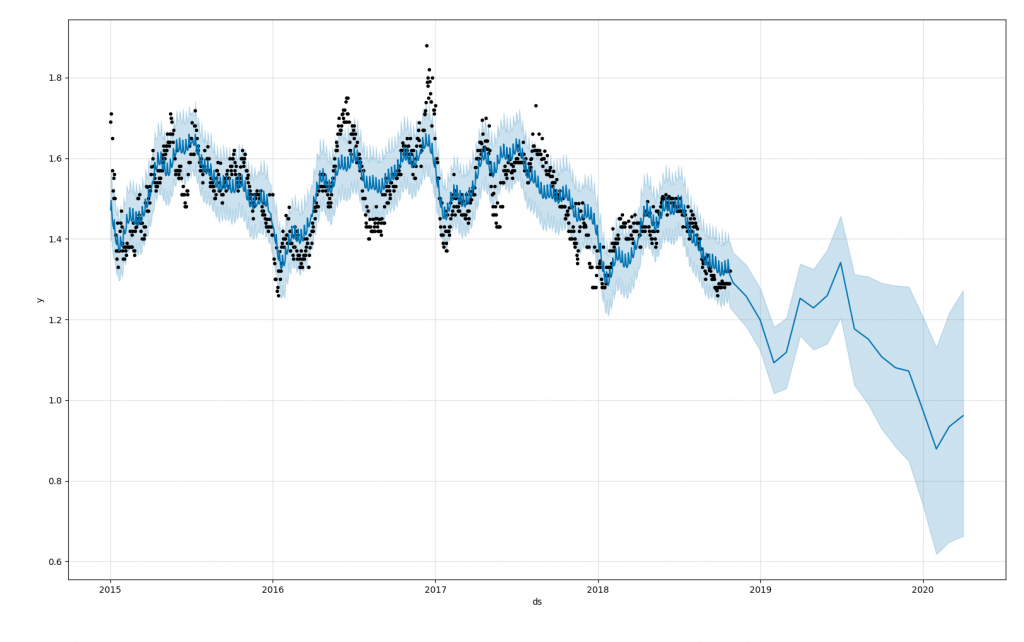
\includegraphics[width=\textwidth,height=0.8\textheight,keepaspectratio]{timeseries_forecast.png}
\end{frame}

%Folie 3
%TabPFN for time series data
\begin{frame}
\frametitle{Time series forecasting with TabPFN}
\begin{itemize}
    \item time series data is similar to tabular data
    %TODO vielleicht hier doch tabelle aus time series data von unteren folien
    % hier beispiel zeigen mit tabelle

    \item TabPFN-TS handles this task very well

    \item applies an additional featurization to the time series data to add 28 new features

    \item achieves top-rank performance on various time series benchmarks
\end{itemize}
\end{frame}
%Folie 4
% Finetuning und continued pretraining
\begin{frame}
    \frametitle{Enhancing performance of a pretrained model}
    \begin{itemize}
    \item But can we enhance the performance of this model?

    \item Two methods:
    \begin{itemize}
        \item finetuning

        \item continued pretraining
    \end{itemize}
    \item RealTabPFN finetuned on multiple dataset and yield superior downstream accuracy
    \end{itemize}
\end{frame}

\begin{frame}
\frametitle{Abstract}
% TabPFN performes well on time series data with the right encoding (see TabPFN-TS paper)

We evaluated three methods to presumably enhance its performance on time series data

\begin{itemize}
\item Finetuning on one dataset
\item Finetuning on multiple datasets
\item Continued Pretraining with synthetic data from a prior developed
\end{itemize}
\end{frame}

\begin{frame}
\frametitle{Structure of this thesis}

In our thesis we evaluated four questions

\begin{itemize}
    \item<2-> Can we improve the performance of TabPFN-TS by finetuning on downstream tasks?

    \item<3-> Can we further improve performance by finetuning on multiple datasets similar to RealTabPFN?

    \item<4-> Can we continue pre-training TabPFN for time series with a prior that generates time series data (and does it improve performance)?

    \item<5-> Which one of the following models performs best on various high-scale benchmarks: TabPFN-TS, finetuned TabPFN-TS, or continued pre-trained TabPFN-TS?
\end{itemize}
\end{frame}

\begin{frame}
\frametitle{Structure of this thesis}

In our thesis we evaluated four questions

\begin{itemize}
    \item \textbf{Can we improve the performance of TabPFN-TS by finetuning on downstream tasks?}

    \item Can we further improve performance by finetuning on multiple datasets similar to RealTabPFN?

    \item Can we continue pre-training TabPFN for time series with a prior that generates time series data (and does it improve performance)?

    \item Which one of the following models performs best on various high-scale benchmarks: TabPFN-TS, finetuned TabPFN-TS, or continued pre-trained TabPFN-TS?
\end{itemize}
\end{frame}

\begin{frame}
\frametitle{Structure of this thesis}

In our thesis we evaluated four questions

\begin{itemize}
    \item \textbf{Can we improve the performance of TabPFN-TS by finetuning on downstream tasks?}

    \item Can we further improve performance by finetuning on multiple datasets similar to RealTabPFN?

    \item Can we continue pre-training TabPFN for time series with a prior that generates time series data (and does it improve performance)?

    \item \textbf{Which one of the following models performs best on various high-scale benchmarks: TabPFN-TS, finetuned TabPFN-TS, or continued pre-trained TabPFN-TS?}
\end{itemize}
\end{frame}

\begin{frame}
\frametitle{Abstract}
    Our Results show that:

    \begin{itemize}
        \item Single Finetuning is especially dependent on dataset characteristics

        \item Multi Finetuning additionally showed good generalization results

        \item Continued Pretraining did not generalize as expected and was the worst of the three methods

    \end{itemize}
    %\item All methods showed promising but not decisive results TODO
\end{frame}

\begin{frame}
\frametitle{Structure of this presentation}
    \begin{itemize}
        \item Background
        \item Single Finetuning
        \item Conclusion
    \end{itemize}
\end{frame}
%Folie 5
% Welche Fragen haben wir evaluiert

\section{Background}
%Folie 1 Time series forecasting
\begin{frame}{Time series}

\begin{columns}[T]

\column{0.58\textwidth}

\textbf{Time Series Definition}

\vspace{0.2cm}

\[
X = \{x_1, x_2, \dots, x_n\} \in \mathbb{R}^{d \times n}
\]
\pause
\[
x_t = t_t + z_t + s_t + \epsilon_t
\]

\pause
\centering
\textit{or}
\[
x_t = t_t \cdot z_t \cdot s_t \cdot \epsilon_t
\]
\begin{align*}
t_t &:\ \text{trend component} & z_t &:\ \text{cyclic component} \\
s_t &:\ \text{seasonal component} & \epsilon_t &:\ \text{noise component}\\
\end{align*}

\column{0.42\textwidth}

\pause
\centering
\textbf{TS as Tabular Data}

\vspace{0.3cm}

\begin{tabular}{cc}
\toprule
Timestamp $t$ & Observation $x_t$ \\
\midrule
2024-01-01 & 21.3 \\
2024-01-02 & 22.1 \\
2024-01-03 & 20.8 \\
2024-01-04 & 23.4 \\
2024-01-05 & 24.0 \\
\bottomrule
\end{tabular}

\end{columns}
\end{frame}
%Folie 3 Time series benchmark (GIFT Eval) (vielleicht hier noch eine folge für die drei split(train, val, test))
\begin{frame}{GIFT-Eval}

\textbf{G}eneral T\textbf{I}me Series
\textbf{F}orecas\textbf{T}ing Model
\textbf{Eval}uation

\vspace{0.3cm}

\begin{columns}[T]

\column{0.5\textwidth}
\centering
\includegraphics<2->[width=\textwidth,height=0.7\textheight,keepaspectratio]{gift_eval2.png}

\column{0.5\textwidth}
\centering
\includegraphics<3->[width=\textwidth,height=0.6\textheight,keepaspectratio]{gift_eval1.png}

\end{columns}
\end{frame}

%Folie 6 Prior fitted networks (vielleicht 2 folien eher 1 weil sehr theoretisch und für vortrag nicht sehr relevant)
\iffalse
\begin{frame}
\frametitle{PFN - Prior Fitted Networks}
    - transformer based architecture

    - trains on artificial tasks generated by a prior

    - approximates posterior predictive distribution $p(y | x, D) = \int_{t} p(y|x, t)p(t, D)$

    - prior is a generative process used to produce large amounts of training data that imitates real-world data
\end{frame}
\fi

\begin{frame}
\frametitle{TabPFN}
    \begin{itemize}
        \item prior fitted network
        \item trains on artificial tabular training tasks
    \end{itemize}
    \centering
    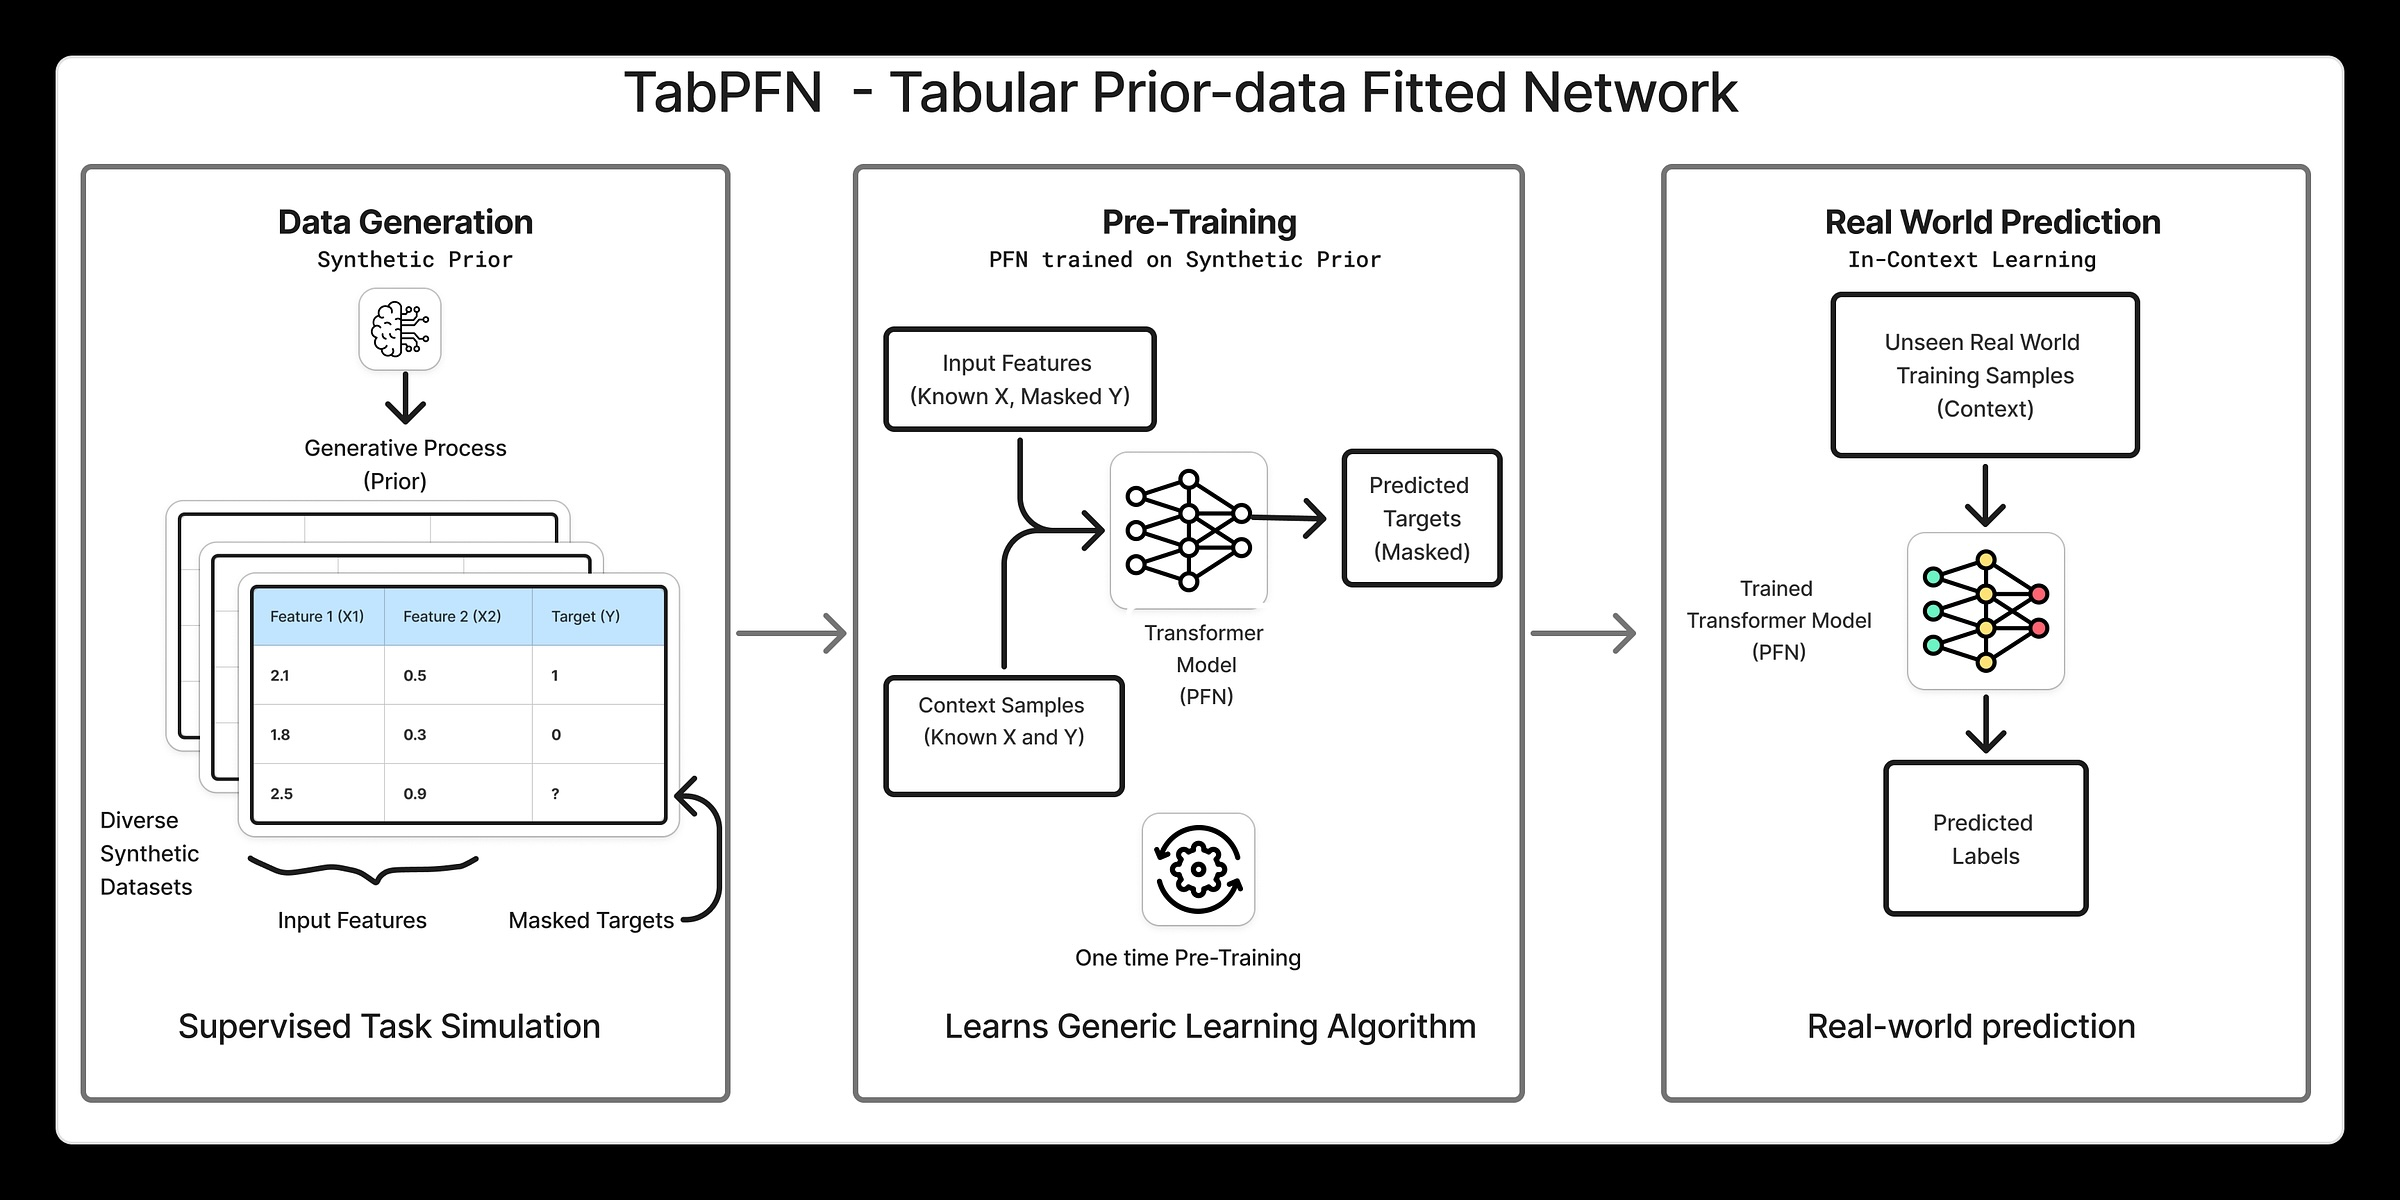
\includegraphics[width=\textwidth,height=0.6\textheight,keepaspectratio]{tabpfn.jpg}
    % important!!: Fitting and prediction is done in same forward pass
\end{frame}

%Folie 9 ForecastPFN Prior einmal kurz und eine Folie mit Beispiel time series. (Vielleicht mehrere auf einer folie für konsistenz)
\begin{frame}{ForecastPFN Prior}

\begin{columns}[T]

\column{0.38\textwidth}

\vspace{0.5cm}

\begin{itemize}
    \item<1-> Used for training ForecastPFN
    \item<2-> Generates synthetic time series data
    \item<3-> We use it for continued pretraining
\end{itemize}

\column{0.62\textwidth}

\centering
\includegraphics<1->[width=\textwidth,height=0.75\textheight,keepaspectratio]
{forecastpfn_example_ts.png}

\end{columns}

\end{frame}

%Folie 7 TabPFN noch mal besser erklären(vielleicht 2 Folien)

%Folie 8 TabPFN-TS einmal featuritzation erklären
\begin{frame}
\frametitle{TabPFN-TS}
    - uses advanced featurization

    - state-of-the-art in covariate-informed forecasting

    - has competitive accuracy in univariate time series forecasting


\end{frame}

%Folie 10 RealTabPFN

% TODO vielleicht noch eine Folie zu finetuning an sich und continued pretraining
\section{Finetuning}
\begin{frame}
\frametitle{Experimental Setup}
    - Code from Lennart Puruckers repository "finetune-tabpfn-v2"

    - data loading with \textbf{code} from \textbf{GIFT Eval}

    - transformation with featurization code from TabPFN-TS

    - no HP search $\rightarrow$ 54 HP config for finetuning $\rightarrow$ take 5 best configurations

    - evaluation script from GIFT Eval
\end{frame}

\begin{frame}
\frametitle{Single Finetuning Results}
\centering
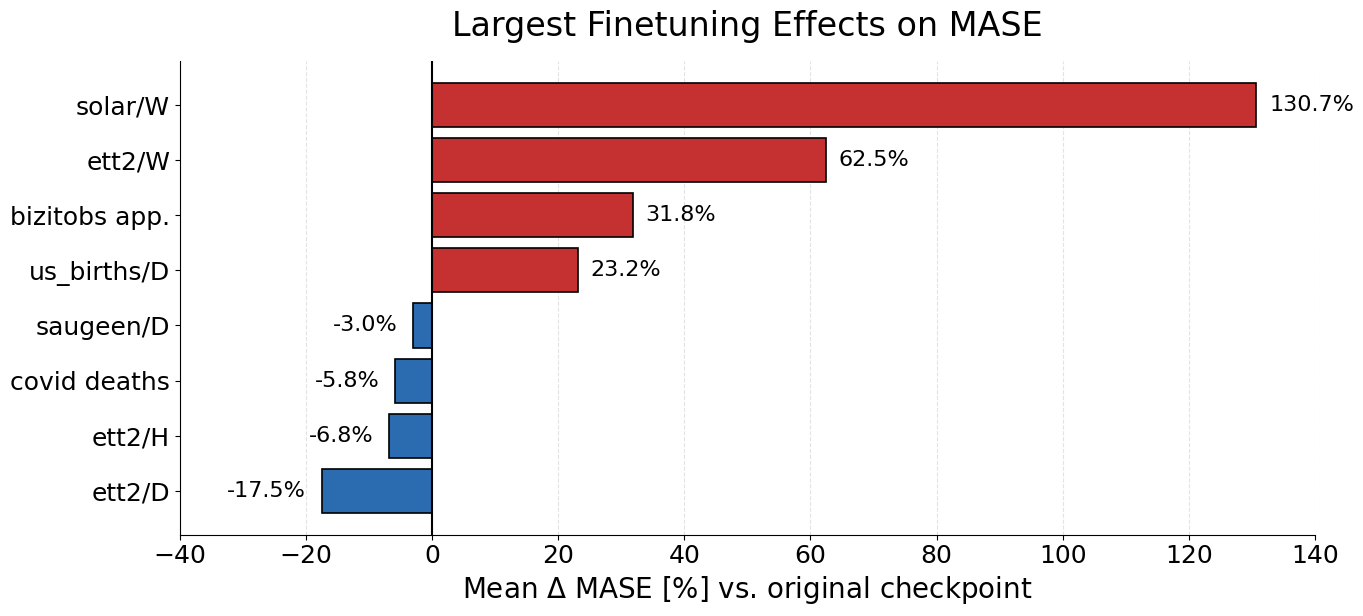
\includegraphics[width=\textwidth,height=0.8\textheight,keepaspectratio]{single_results.png}
\end{frame}

\section{Can we improve the performance of TabPFN-TS by finetuning on downstream tasks?}
\begin{frame}{Context Length and Number of Time Series}

\begin{columns}[T]

\column{0.5\textwidth}
\centering
\includegraphics<1->[width=\textwidth,height=0.7\textheight,keepaspectratio]
{plot1_score_series.pdf}

\vspace{0.2cm}

\only<1->{\small Score Series}

\column{0.5\textwidth}
\centering
\includegraphics<2->[width=\textwidth,height=0.7\textheight,keepaspectratio]
{plot2_context_vs_series.pdf}

\vspace{0.2cm}

\only<2->{\small Context vs Series}

\end{columns}

\end{frame}

\begin{frame}{Intermittent Data}

\begin{columns}[T]

\column{0.38\textwidth}

\vspace{0.5cm}

\begin{itemize}
    \item<1-> Example of a difficult structure for finetuning
    \item<2-> Many zero values
    \item<3-> Sudden spikes
    \item<4-> Hard to generalize
\end{itemize}

\column{0.62\textwidth}

\centering
\includegraphics<1->[width=\textwidth,height=0.75\textheight,keepaspectratio]
{bizitobs_service_plot.png}

\end{columns}

\end{frame}
%Folie 1 MSE und Evaluation korrelieren nicht so wie gedacht
%Folie 2 Number of observation and in one dataset
%Folie 3 Exception exmaples with noisy and intermittent data
\section{Conclusion}

\begin{frame}
\frametitle{Conclusion}
    \begin{itemize}
        \item finetuning on a single dataset works but is dependent on
        \begin{itemize}
            \item number of time series
            \item context length
            \item dataset structure
            \begin{itemize}
                \item clear patterns are beneficial
                \item noisy or intermittent data remain challenging
            \end{itemize}
        \end{itemize}
    \end{itemize}
\end{frame}

\begin{frame}{Other Two Methods}

\textbf{Multi Finetuning}
\begin{itemize}
    \item<1-> Clustering into three categories
    \begin{itemize}
        \item<2-> Small only led to deterioration
        \item<3-> Medium showed the best generalization results
        \item<4-> Large showed acceptable results
    \end{itemize}
\end{itemize}

\vspace{0.5cm}

\uncover<5->{
\textbf{Continued Pretraining}
}
\begin{itemize}
    \item<6-> Very \textbf{heterogeneous} improvements
    \item<7-> Mostly \textbf{deterioration}
\end{itemize}

\end{frame}
%1. Folie Tabelle mit allen Ergebnissen und Methoden zeigen
%2. Folie Finetuning highly dataset dependent
%3. Folie Validation nicht so gut. sehr wahrscheinlich wegen MSE und MASE
%4. Multi Finetuning can lead to better generalization but in small context length it only leads to deterioration
%5. Continued Pretraining
%6. Final Conclusion

\begin{frame}
\frametitle{Limitations}
    \begin{itemize}
        \item<1-> datasets only provide \textbf{limited perspective}
        \item<2-> not all \textbf{evaluation scores} could be reproduced
        \item<3-> \textbf{mismatch} between validation loss and evaluation metric
        \item<4-> computational limitations
        \item<5-> \textbf{TabPFN 2.5} was released during the thesis
    \end{itemize}
\end{frame}

\begin{frame}
\frametitle{Outlook}
    \begin{itemize}
        \item<1-> improving \textbf{evaluation procedure}
        \item<2-> \textbf{dataset selection} for multi-dataset finetuning
        \item<3-> systematic \textbf{hyperparameter search}
        \item<4-> effect of newer model versions (TabPFN 2.5)
        \item<5-> sensitivity of \textbf{prior-based continued pretraining}
    \end{itemize}
\end{frame}

\begin{frame}
\frametitle{Conclusion}
    \textbf{Which one of the following models performs best on various high-scale benchmarks: TabPFN-TS, finetuned TabPFN-TS, or continued pre-trained TabPFN-TS?}
    \begin{itemize}
        \item no finetuning strategy dominates all scenarios
        \item based on use case for finetuning
        \item based on dataset availability structure and quality of the underlying data
        \begin{itemize}
            \item not much available data $\rightarrow$ Prior
            \item not much real world data but many different datasets $\rightarrow$ Multi finetuning
            \item much real world datasets and many time series in it $\rightarrow$ Single finetuning
        \end{itemize}
    \end{itemize}
\end{frame}

\section{Thank you for your Attention}
\section{Backup Slides}
\begin{frame}
\frametitle{TabPFN-TS Featurization}
    - Running Index: $\Phi_{index}(t) = t \in \mathbb{R}$

    - Calendar Features: $\Phi_{cal}(t)=\left(cos\left(\frac{2 \pi t}{P_1}\right), sin\left(\frac{2 \pi t}{P_1}\right), …, cos\left(\frac{2 \pi t}{P_8}\right), sin\left(\frac{2 \pi t}{P_8}\right), year(t)\right) \in \mathbb{R}^{17}$ %TODO hier vielleicht noch second of minute etc

    - Automatic Season Features: $\Phi_{auto}(t) = (cos(2\pi f_1 t), sin(2 \pi f_1 t), …, cos(2\pi f_k t), sin(2 \pi f_k t)) \in \mathbb{R}^{2k}$

    - Time-varying Covariates (when available): $z_{1:C+H} = [z_1, …, z_{C+H}]$ where $z_t \in \mathbb{R}^{D_{z}}$ represents $D_z$ external variables observed at time \textbf{t}

\end{frame}
\end{document}
